\subsection{Построение и аппроксимация зависимости \(\sin\varphi_m\) от \(m\)}

Для каждой спектральной линии (\(i=1\) — красная, \(i=2\) — зелёная, \(i=3\) — фиолетовая) были рассчитаны точки
\[
	\bigl(m,\;\sin\varphi_{m,i}\bigr),
	\quad m=\pm1,\pm2,\pm3,
\]
и построены аппроксимирующие прямые
\[
	\sin\varphi = a_i\,m
\]
методом наименьших квадратов без свободного члена. Ниже приведены соответствующие графики.

\begin{figure}[H]
	\centering
	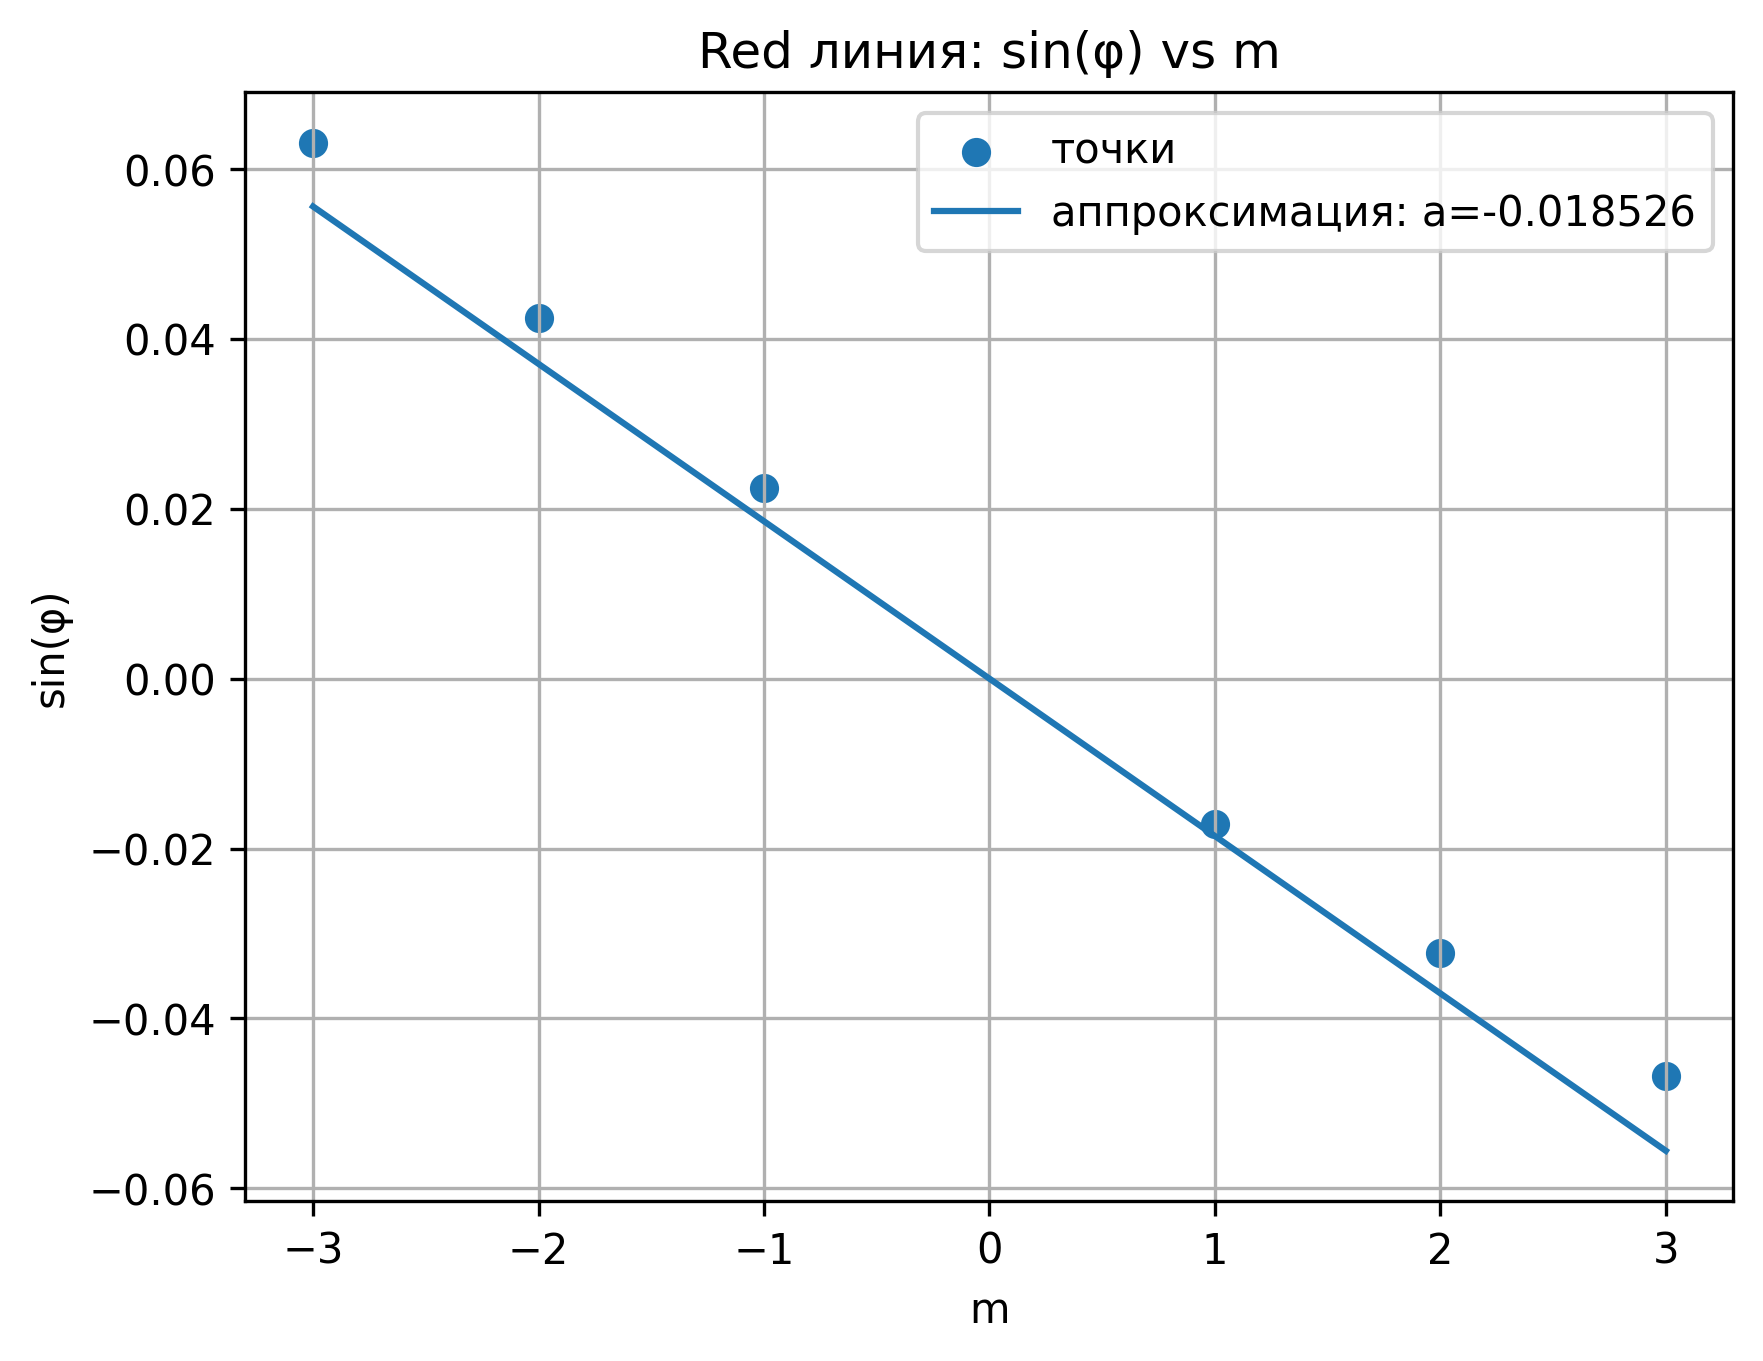
\includegraphics[width=0.7\textwidth]{images/red_fit.png}
	\caption{Красная линия: \(\sin\varphi\) vs.\ \(m\) и аппроксимация \(a_1\,m\).}
	\label{fig:sinphi-red}
\end{figure}

\begin{figure}[H]
	\centering
	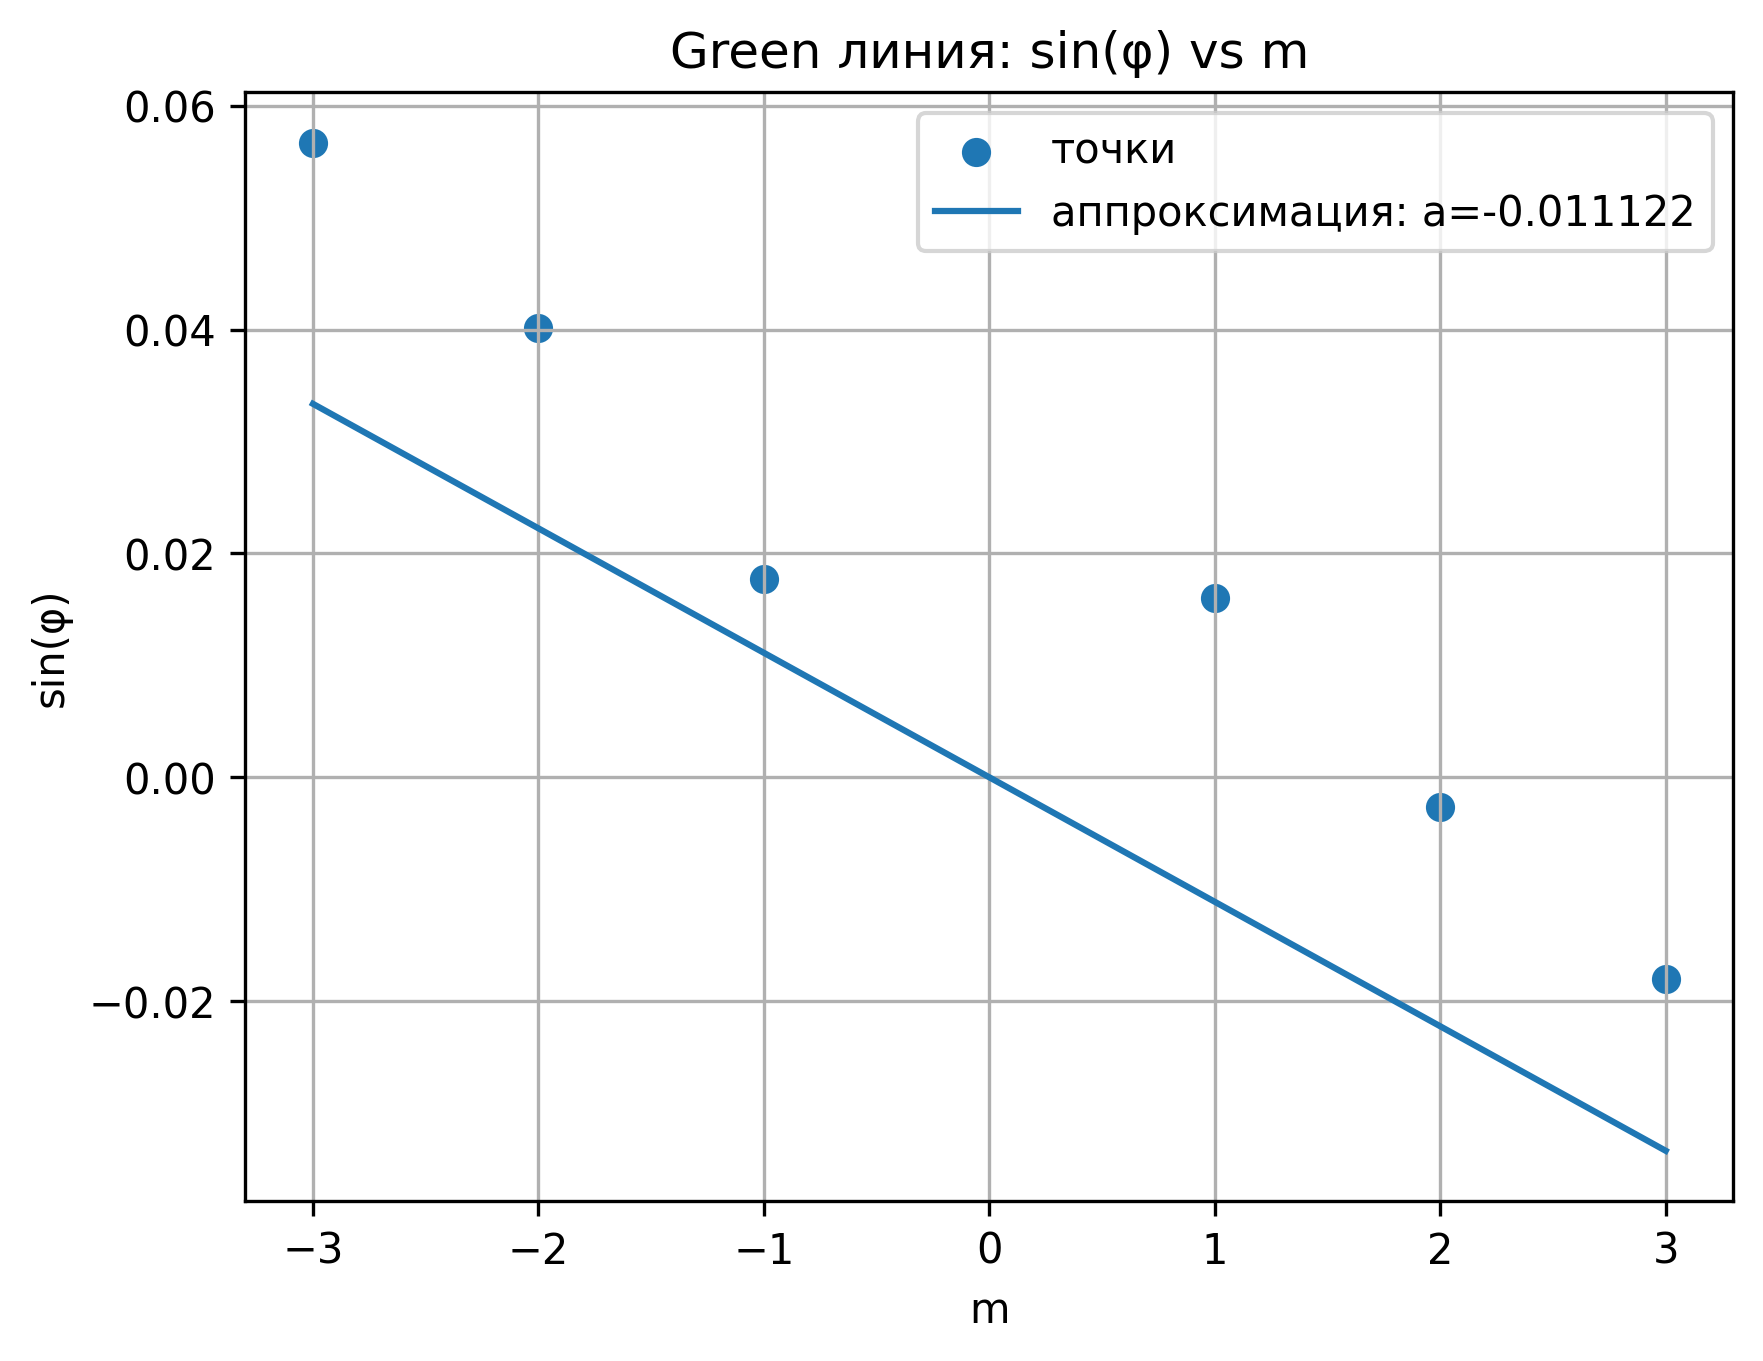
\includegraphics[width=0.7\textwidth]{images/green_fit.png}
	\caption{Зелёная линия: \(\sin\varphi\) vs.\ \(m\) и аппроксимация \(a_2\,m\).}
	\label{fig:sinphi-green}
\end{figure}

\begin{figure}[H]
	\centering
	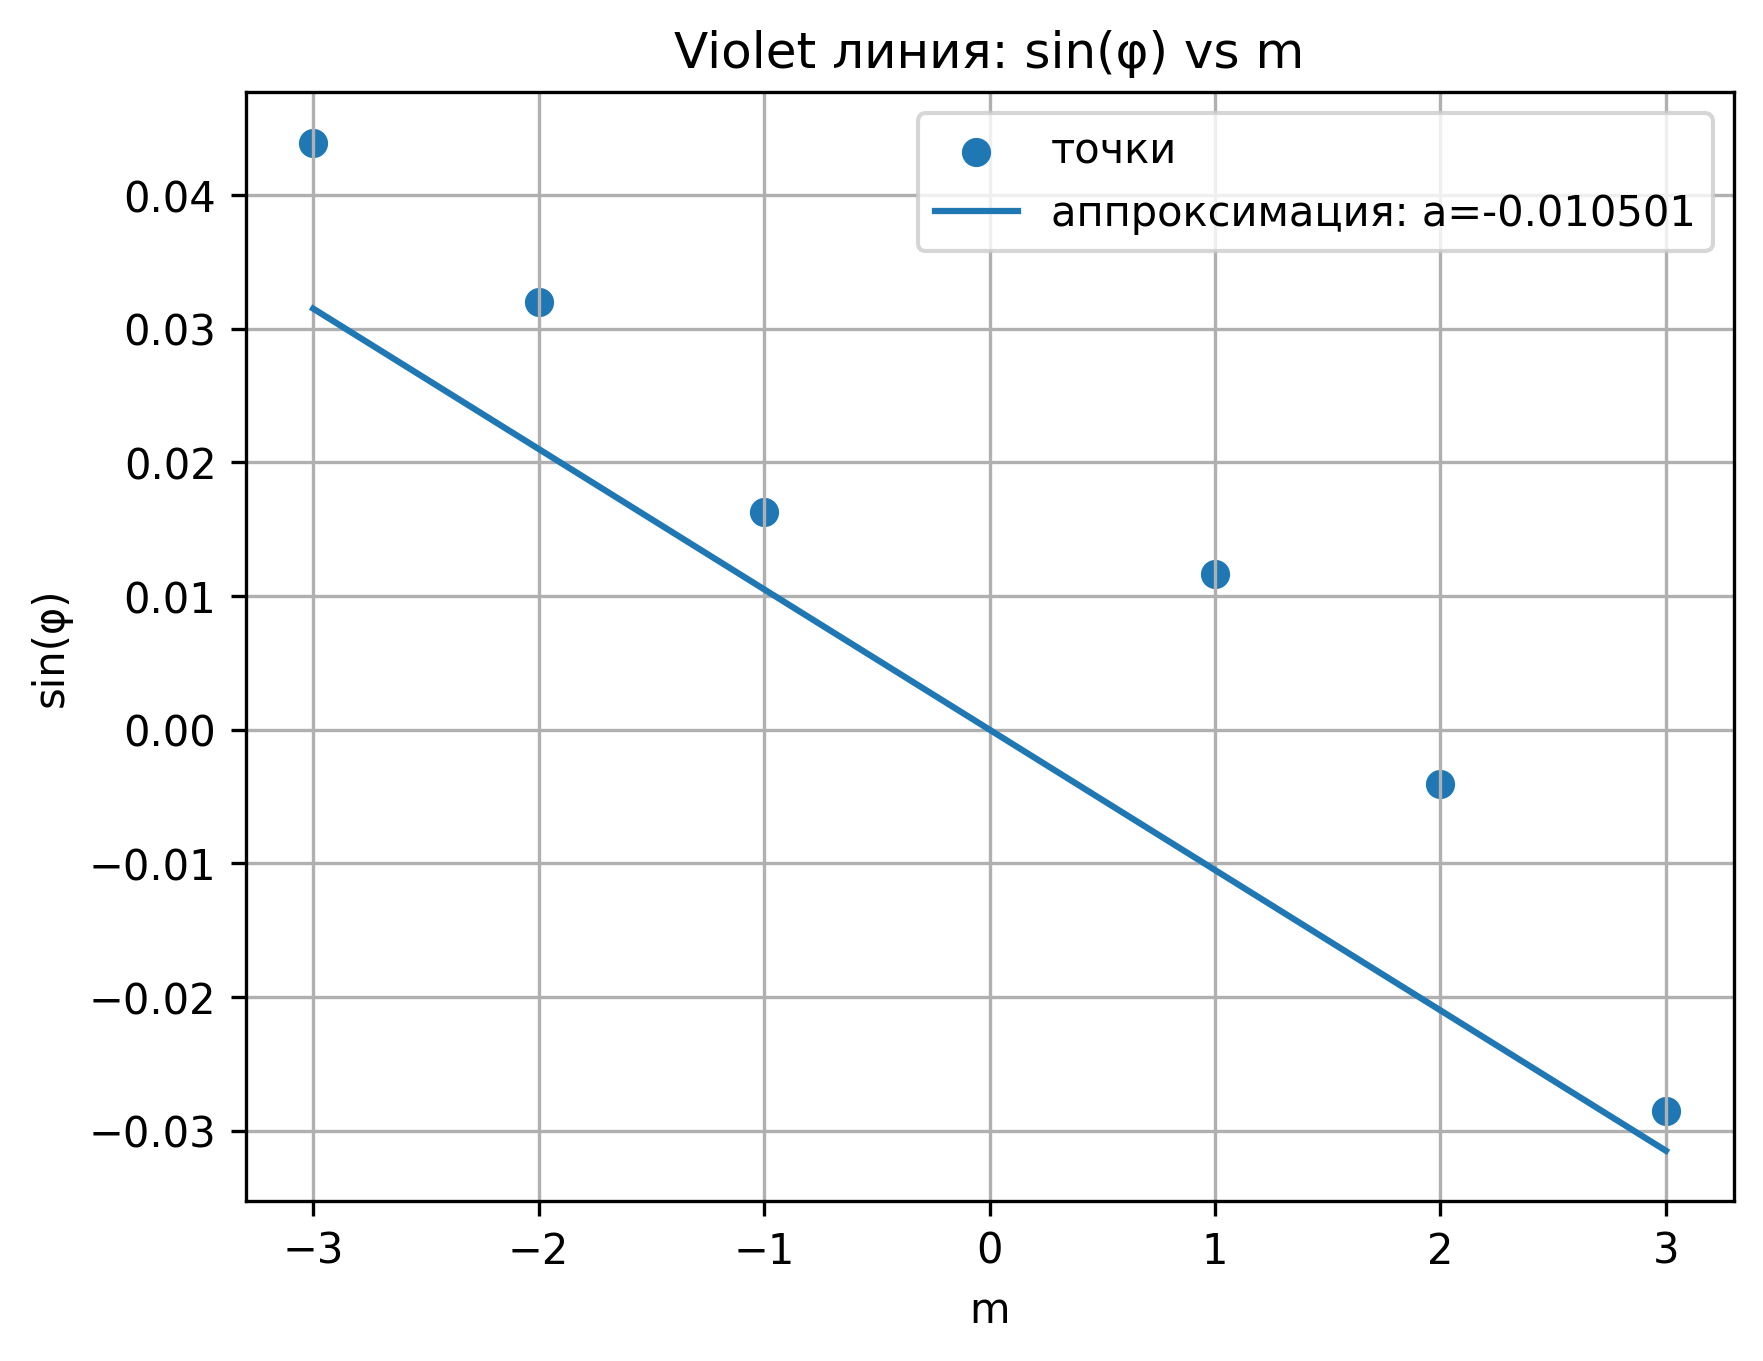
\includegraphics[width=0.7\textwidth]{images/violet_fit.png}
	\caption{Фиолетовая линия: \(\sin\varphi\) vs.\ \(m\) и аппроксимация \(a_3\,m\).}
	\label{fig:sinphi-violet}
\end{figure}
